\subsection{Student Intake Explains Little of the Field Differences}
\label{sec:res-confounders}

We find little evidence that the available intake measures account for the shared field pattern. Across 29 fields, the association between national admission grade and the field effect has slope 0.05 ($p=0.26$). In Figure~\ref{fig:confounders}, the points remain close to the no-change line when we add admission grade and size: before and after effects correlate 0.99, and their spread remains about 0.31 grade points. The figure covers 8,043 observations from 47 public universities. However, admission grades distinguish only five broad branches for 29 fields; they cannot separate intake within a branch, so the near-identity partly reflects this weak measurement. In the nested control analysis, the admission coefficient is 0.056 points per standard deviation ($p<0.001$), suggesting a small positive intake association without explaining away the field pattern.

\begin{figure}[t]
  \centering
  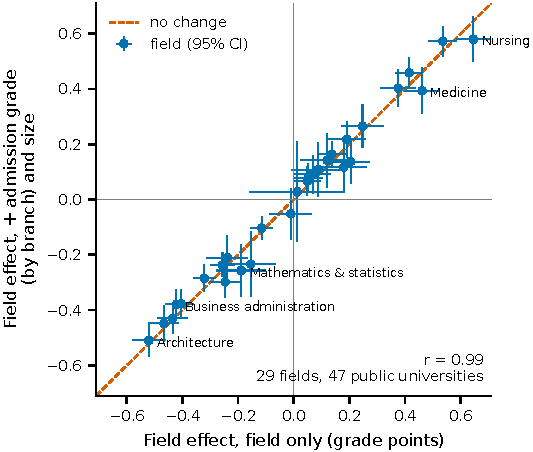
\includegraphics[width=0.92\linewidth]{fig3_confounders}
  \caption{Field effects before (horizontal axis) and after (vertical axis) adjustment for admission grade and size, in grade points on the Spanish 5--10 scale; SIIU, 8,043 records from 47 public universities. Bars show 95\% confidence intervals clustered by university; the dashed red line denotes no change. Admission grades identify only five broad branches, limiting adjustment within branches. Original figure; data from SIIU.}
  \label{fig:confounders}
\end{figure}

We obtained a similar conclusion using individual Portuguese entry grades. The gap between the highest- and lowest-graded degrees decreases from 1.51 to 1.30 points on the 0--20 scale after standardised entry grades and background controls. Degree remains jointly significant ($F=38.1$, 14 degrees of freedom, $p<0.001$). Most of the gap therefore remains even where intake is measured individually. We interpret this as an adjusted association, not evidence that equally able students would necessarily receive different grades if assigned to different degrees.

We found more attenuation when we added dropout: the spread falls from 0.31 to 0.24 points, and the effects correlate 0.95 with the original estimates. Higher dropout is associated with lower grades, but the direction is unresolved. Stricter grading may drive departures, while the remaining graduates are a selected group. We therefore report this specification separately rather than using it to claim that dropout causes the observed differences.
